\chapter{Grammaires} % (fold)
\label{cha:grammaires}


\section{Comment définir un langage} % (fold)
\label{sec:comment_d_finir_un_langage}

\begin{itemize}
	\item On peut définir un langage par une phrase en Français.
	
	\paragraph{Exemple} % (fold)
	\label{par:exemple}

	$\mathcal{L}_p$ est le langage de tous les mots de longueur pair sur un l'alphabet $\{a,b\}$\\

	% paragraph exemple (end)


	\item Si le langage est fini, on peut donner, énumérer tous ses éléments(Définition en extension).

	\paragraph{Exemple} % (fold)
	\label{par:exemple}

	$A=\{\epsilon, a, bb, abab\}$\\
	
	% paragraph exemple (end)


	\item Un langage peut être défini par une propriété caractéristique de ses mots(Définition en extension).

	\paragraph{Exemple} % (fold)
	\label{par:exemple}

	$\mathcal{L}_p = \{w \in \{a,b\}^* \mid \forall n \in \mathbb{N}, \left|w\right|=2*n\}$\\
	
	% paragraph exemple (end)


	\item Un langage peut être défini à partir d'un autre langage par des opérations ensemblistes tels que Union, Intersection, Différence, Complémentation, Étoile, ...\\


	\item Un langage peut se définir de manière opérationnelle en donnant un algorithme de décision (fonction booléenne), qui prend en entré un mot quelconque et indique si le mot fait parti ou non du langage. La notion d'automate donne un formalisme opérationnel pour décider de l'appartenance d'un mot à un langage (reconnaître, accepter un mot).

	\paragraph{Exemple} % (fold)
	\label{par:exemple}

	Est ce que un mot $w \in \mathcal(L)_p$. On peut écrire un algorithme qui compte le nombre de caractères du mot $w$ et vérifie si le résultat est paire ou on se contente d'un automate à 2 états qui compte le nombre de symbole modulo 2.\\
	
	% paragraph exemple (end)


	\item On peut donner un procéder de génération de l'ensemble des mots du langage. La notion de grammaire est un formalisme qui permet de générer, engendrer l'ensemble des mots d'un langage.\\

	\paragraph{Exemples} % (fold)
	\label{par:exemples}

	\begin{itemize}
		\item On peut définir indirectement le langage $\mathcal{L}_p$ avec les règles suivantes :\\
		$\epsilon \in \mathcal{L}_p$.\\
		Si un mot $w \in \mathcal{L}_p$, alors $aaw \in \mathcal{L}_p$, $baw \in \mathcal{L}_p$, $abw \in \mathcal{L}_p$ et $bbw \in \mathcal{L}_p$.

		\item Soit $\mathcal{A}$ un langage défini sur l'alphabet $\Sigma = \{a,b\}$, on peut avoir :\\
		$\epsilon \in \mathcal{A}$.\\
		Si le mot $w \in \mathcal{A}$ alors $awb \in \mathcal{A}$.
		$\mathcal{A} = \{w \in \{a,b\} \mid \exists \mathbb{N}, w=a^nb^n\}$
	\end{itemize}

	% paragraph exemples (end)


\end{itemize}

% section comment_d_finir_un_langage (end)


\section{Grammaire formelle} % (fold)
\label{sec:grammaire_formelle}

Une grammaire est un ensemble de règles qui permettent de produire, générer, engendre, les mots d'un langage.


\paragraph{Définition} % (fold)
\label{par:d_finition}

Une grammaire est un quadruplet $(\Sigma,N,P,S)$ où :

\begin{itemize}
	\item $\Sigma$ est un alphabet, un ensemble fini de symboles terminaux.
	\item $N$ est un ensemble fini de symboles non terminaux, on a $N$ et $\Sigma$ disjoints.
	\item $P$ est un ensemble fini de règles de production.
	\item $S \in N$ est l'axiome, ou le symbole initial.
\end{itemize}

% paragraph d_finition (end)


\paragraph{Remarque} % (fold)
\label{par:remarque}

Si $\alpha \rightarrow \beta_1$ et $\alpha \rightarrow \beta_2$ sont 2 règles de production, on peut écrire de manière plus concise les 2 règles sous la forme $a \rightarrow \beta_1 \mid \beta_2$.

% paragraph remarque (end)


\paragraph{Exemples} % (fold)
\label{par:exemples}

\begin{itemize}
	\item Soit la grammaire suivante, $(\{a,b\},\{S\},\{S \rightarrow\ aaS, S \rightarrow abS, S \rightarrow baS, S \rightarrow bbS, S \rightarrow \epsilon\},S)$ est une grammaire qui engendre le langage $\mathcal{L}_p$.

	\item La grammaire suivante, $(\{a,b\},\{S,A,B\},\{S \rightarrow A \mid B, A\rightarrow aA \mid a, B \rightarrow bB\mid b\},S)$, a 6 règles de productions et est un langage non vide dont les mots n'ont que des $a$ ou que des $b$.
\end{itemize}

% paragraph exemples (end)


\paragraph{Définition} % (fold)
\label{par:d_finition}

Soient la grammaire $G = (\Sigma,N,P,S)$ et $(\alpha,\beta) \in (\Sigma \cup N)^*$, on a :

\begin{itemize}
	\item $\beta$ dérive en une étape de $\alpha$, noté $\alpha \Rightarrow \beta$ s'il existe $x \rightarrow y \in P$ et s'il existe $(u,v) \in (\Sigma \cup N)^*$ tel que :\\
	$\alpha = uxv$ et $\beta = uyv$

	\item $\alpha_k$ dérive de $\alpha_0$ en k étapes, noté $\alpha_0 \Rightarrow^k \alpha_k$ s'il existe $(\alpha_1,\alpha_2,...,\alpha_(k-1)$ tel que quelque soit $i < k$, $\alpha_{i+1}$ dérive en une étape de $\alpha_i$.
\end{itemize}

% paragraph d_finition (end)


\paragraph{Exemple} % (fold)
\label{par:exemple}

Soit la grammaire suivante $(\{a,b\},\{S,A,B\},\{S \rightarrow A \mid B, A\rightarrow aA \mid a, B \rightarrow bB\mid b\},S)$.\\
Le mot $aAabASSABba$ dérive en une étape de $aAAbASSABba$, vue que l'on peut prendre $u=aA$, $x=A$, $v=bASSABba$ et $y=a$.\\
Le mot $aaa$ est dérivé en 4 étapes de $S$, grâce à la décomposition suivante :\\
$S \Rightarrow A$, $A \Rightarrow aA$, $aA \Rightarrow aaA$, $aaA \Rightarrow aaa$, on peut donc écrire $S \Rightarrow^4 aaa$.

% paragraph exemple (end)


\paragraph{Définition} % (fold)
\label{par:d_finition}

On note $\Rightarrow^*$, la clôture réflexive transitive de la relation $\Rightarrow$. $\beta$ dérive de $\alpha$, si $\alpha \Rightarrow^* \beta$ c'est-à-dire qu'il existe $k \in \mathbb{N}$, tel que $\alpha \Rightarrow^k \beta$.

% paragraph d_finition (end)


\paragraph{Remarque} % (fold)
\label{par:remarque}

Tout mot dérivé de lui même, avec k=0.\\
Si $\beta$ dérive de $\alpha$, il existe une suite de mots, $\alpha_0, \alpha_1, ... , \alpha_k$ avec $\alpha_0 = \alpha$ et $\alpha_k = \beta$ tel que quelque soit $i < k$, $\alpha_i \Rightarrow \alpha_{i+1}$. Cette suite est appelé dérivation et est noté $\alpha_0 \Rightarrow \alpha_1 \Rightarrow ... \Rightarrow \alpha_k$.

% paragraph remarque (end)


\paragraph{Définition} % (fold)
\label{par:d_finition}

Soit une grammaire $G=(\Sigma,N,P,S)$, le langage engendré par un non terminal $X \in N$, noté $\mathcal{L}(X)$ et $\mathcal{L}(X)=\{wG \in \Sigma^* \mid X \Rightarrow^* w \}$.\\
Si le mot $w$ dérive de $S$ et $w \in \Sigma^*$, alors $w$ est un mot engendré par $G$. Le langage engendré par $G$, noté $\mathcal{L}(G)$, est $\mathcal{L}(G)=\mathcal{L}(S)=\{w \in \Sigma^* \mid S \Rightarrow w\}.$\\
On dit que 2 grammaires sont équivalentes si elles engendrent le même langage.

% paragraph d_finition (end)


\paragraph{Exemples} % (fold)
\label{par:exemples}

Soient les 2 langages suivants, $\mathcal{L}(A)=\{a^n \mid n > 0\}$ et $\mathcal{L}(B)=\{b^n \mid n > 0\}$, alors on peut avoir le langage suivant : $\mathcal{L}(G) = \mathcal{L}(S) = \mathcal{L}(A) \cup \mathcal{L}(B)$.

% paragraph exemples (end)


% section grammaire_formelle (end)


\section{Hiérarchie de Chomsky} % (fold)
\label{sec:hi_rarchie_de_chomsky}

La Hiérarchie ou la Classification permet de classer un type selon la forme des règles de production d'une grammaire. Ainsi, on peut associé une grammaire à un type de la Hiérarchie. Il existe 4 types :

\begin{itemize}
	\item Type 0 : Ce sont des grammaires général, il y a aucune restrictions sur les règles.
	\item Type 1 : Ce sont des grammaires contextuelles (ou context-sensitive), toutes les règles sont de la forme $\alpha_gA\alpha_d \rightarrow \alpha_g\beta\alpha_g$ avec $\alpha_g,\alpha_d \in (\Sigma \cup N)^*$, $A \in N$, $\beta \in (\Sigma \in N)^+$.
	\item Type 2 : Ce sont des grammaires algébriques (ou context-free), et ont des règles de productions de la forme $A \rightarrow \beta$ avec $A \in N$ et $\beta \in (\Sigma \cup N)^*$.
	\item Type 3 : Ce sont des grammaires régulières (ou linéaire droite), dont les règles de productions sont de la forme : $A \rightarrow \beta$ avec $A \in N$ et $\beta \in (\Sigma^*(N \cup \{\epsilon\}))$.
\end{itemize}

Si on note $\mathcal{L}_0, \mathcal{L}_1, \mathcal{L}_2, \mathcal{L}_3$, les ensembles de langages engendrés respectivement par les grammaires de type 0, 1, 2 et 3, on a les inclusions stricts suivantes : $\mathcal{L}_3 \subset \mathcal{L}_2 \subset \mathcal{L}_1 \subset \mathcal{L}_0$.

\begin{figure}
\center
\label{maqao}
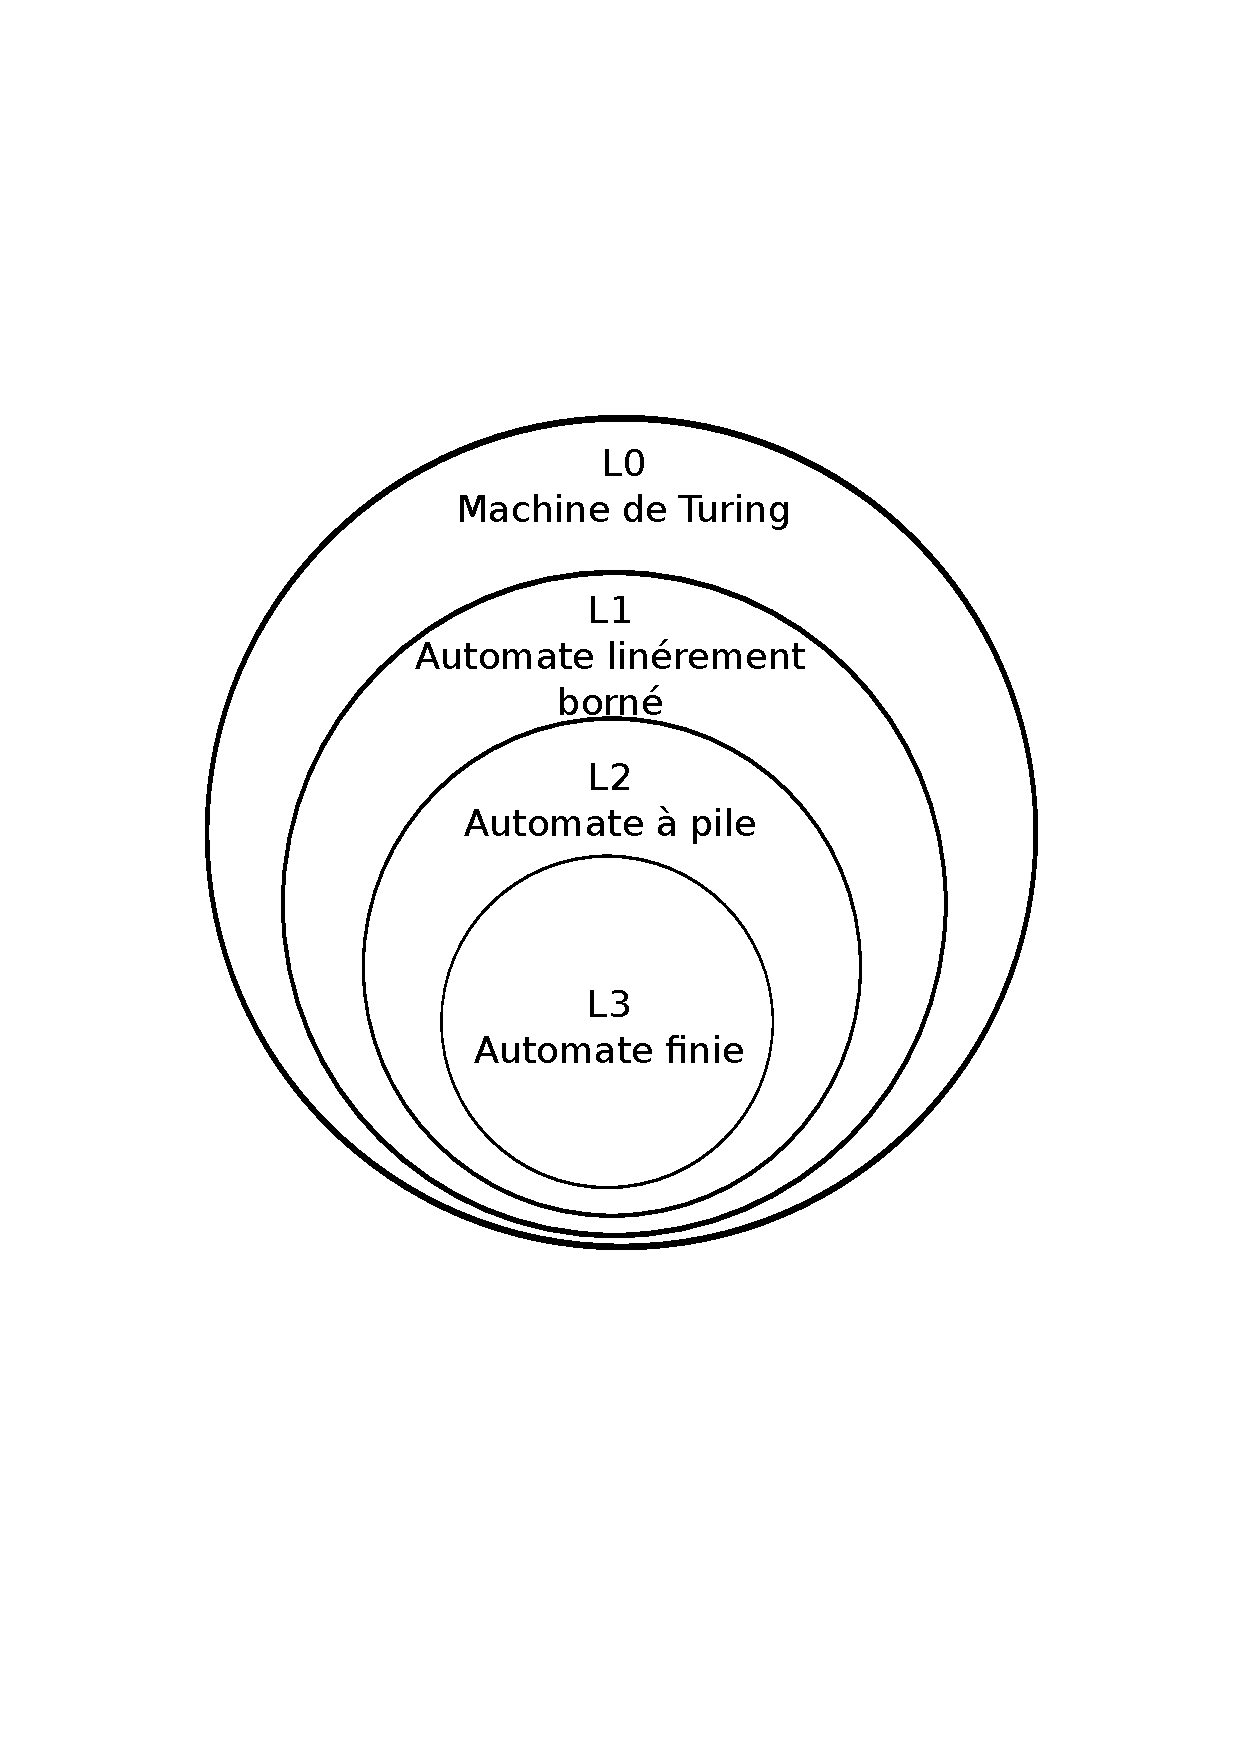
\includegraphics[width=16cm]{part_3/images/hierarchie_chomsky.pdf}
\caption{Hiérarchie de Chomsky}
\end{figure}


\paragraph{Définition} % (fold)
\label{subp:d_finition}

Un langage est de type k, avec $k \in (0,1,2,3)$, s'il existe une grammaire de type k qui l'engendre.
\begin{itemize}
	\item Un langage est régulier s'il est de type 3.
	\item Un langage est algébrique s'il est de type 2.
	\item Un langage est contextuelle s'il est de type 1.
	\item Un langage est récursivement énumérable s'il est de type 0.
\end{itemize}

% paragraph d_finition (end)


\paragraph{Notations} % (fold)
\label{par:notations}

La notation BNF, ou Backus-Naur Forme, est une description d'un langage de programmation. Les terminaux sont les symboles du langages et les non terminaux sont les noms des choses que l'on définit. Les non terminaux sont écrit entre $<>$.

% paragraph notations (end)


\paragraph{Exemple} % (fold)
\label{par:exemple}

Le mot clé $if$ du langage $C++$ a l'une des règles suivantes :\\
$<structure\_if> ::= if\ "(" <conditions> ")"\ "\{" <code> "\}"\ [\ else\ "\{" <code> "\{"\ ]$

% paragraph exemple (end)


% section hi_rarchie_de_chomsky (end)


\section{Grammaires algébriques} % (fold)
\label{sec:grammaires_alg_briques}


\paragraph{Définition} % (fold)
\label{par:d_finition}

Soit une grammaire algébrique $G=(\Sigma, N, P, S)$, une dérivation gauche, respectivement droite, est une dérivation dans laquelle le non terminal dérivé est toujours le plus à gauche, respectivement à droite.

% paragraph d_finition (end)


\paragraph{Définition} % (fold)
\label{par:d_finition}

Un arbre de dérivation est un arbre étiqueté par $\Sigma \cup N \cup \{\epsilon\}$ qui vérifie :

\begin{itemize}
	\item Tout nœud interne, ainsi que la racine, est étiqueté par un non terminal, soit un élément de N.
	\item Si A est l'étiquette d'un nœud $\alpha_1, \alpha_2, ..., \alpha_n$ sont les étiquettes de ses n fils, dans cette arbre, alors $A \rightarrow \alpha_1\alpha_2...\alpha_n \in P$.
\end{itemize}

À tous arbres de dérivations, on peut associer un mot sur $(\Sigma \cup N)^*$ formé des étiquettes des feuilles de l'arbre dans l'ordre dans lequel elles sont visités par un parcours infixe de l'arbre.

% paragraph d_finition (end)


\paragraph{Exemple} % (fold)
\label{par:exemple}

Soit une grammaire algébrique $G=(\{a,b\} , \{S\} , \{S\rightarrow aSbS \mid bSaS \mid \epsilon\} , S)$, on a l'arbre de dérivation suivant :

\begin{center}
	
	\begin{tikzpicture}[level distance=11mm,sibling distance=20mm]
	
	\node {S}
		child{node{a}}
		child{node{S}
			child{node{$\epsilon$}}}
		child{node{b}}
		child{node{S}
			child{node{b}}
			child{node{S}
				child{node{$\epsilon$}}}
			child{node{a}}
			child{node{S}
				child{node{$\epsilon$}}}
			};
	\end{tikzpicture}

\end{center}

On peut avoir plusieurs dérivations pour un mot donné :
\begin{itemize}
	\item $S \Rightarrow aSbS \Rightarrow abS \Rightarrow abbSaS \Rightarrow abbaS \Rightarrow abba$ (Dérivation gauche)
	\item $S \Rightarrow aSbS \Rightarrow aSbbSaS \Rightarrow aSbbaS \Rightarrow abbaS \Rightarrow abba$.
\end{itemize}

% paragraph exemple (end)


\paragraph{Proposition} % (fold)
\label{par:proposition}

Soit une grammaire algébrique $G=(\Sigma,N,P,S)$, avec $A \in N$, alors $A\Rightarrow^* \alpha$ si et seulement s'il existe un arbre de dérivation de racine étiqueté par A et dont le mot associé est $\alpha$.

% paragraph proposition (end)

Le langage engendré par G est l'ensemble des mots sur $\Sigma^*$ associés à des arbres de dérivations de racine étiquette par S (les feuilles sont étiquetées par $\Sigma \cup \{\epsilon\}$).

% section grammaires_alg_briques (end)


\paragraph{Définition} % (fold)
\label{par:d_finition}

La grammaire algébrique G est ambiguë s'il existe $w \in \mathcal{L}(G)$ associés à 2 arbres de dérivations différents partant de l'axiome. Un langage algébrique est ambiguë si toute grammaire qu'il engendre est ambiguë.

% paragraph d_finition (end)


\paragraph{Exemples} % (fold)
\label{par:exemples}

\begin{itemize}
	\item Soit le code suivant :\\
$if(a)\\
if(b)\\
c;\\
else\\
d;$\\

Comment peut-on interpréter ce code avec les 2 règles suivantes :

\begin{itemize}
	\item $if\ (cond)\ instructions ;\ else\ instructions;$
	\item $if\ (cond)\ instructions ;$
\end{itemize}

On obtient alors 2 arbres de dérivations :

\begin{center}
	
	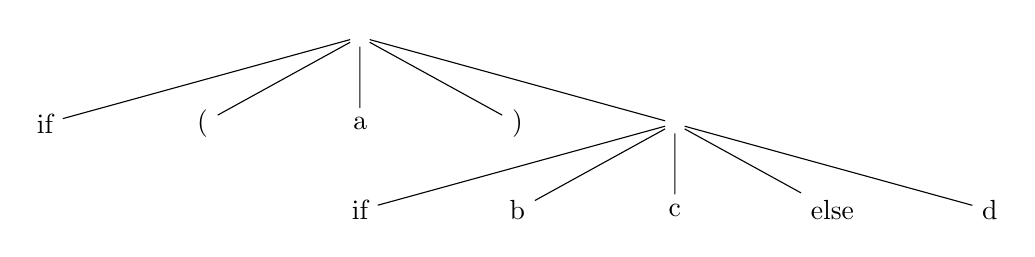
\begin{tikzpicture}[level distance=11mm,sibling distance=20mm]

	\node {}
		child{node{if}}
		child{node{(}}
		child{node{a}}
		child{node{)}}
			child{node{}
				child{node{if}}
				child{node{b}}
				child{node{c}}
				child{node{else}}
				child{node{d}}
			}
		;

	\end{tikzpicture}

\end{center}


\begin{center}
	
	\begin{tikzpicture}[level distance=11mm,sibling distance=20mm]

	\node {}
		child{node{if}}
		child{node{a}}
		child{node{}
			child{node{if}}
			child{node{b}}
			}
		child{node{else}}
		child{node{d}}
	;
	\end{tikzpicture}

\end{center}


\item Soit la grammaire suivante, $G=(\{a,+,*\} , \{S\} , \{S\rightarrow S+S \mid S*S \mid a\} , S)$, pour le mot suivant $a+a*a$ on obtient les arbres suivants :

\begin{center}
	
	\begin{tikzpicture}[level distance=11mm,sibling distance=20mm]

	\node {S}
		child{node{S}
			child{node{a}}
			}
		child{node{+}}
		child{node{S}
			child{node{S}
				child{node{S}
					child{node{a}}
					}
				child{node{*}}
				child{node{S}
					child{node{a}}
					}
				}
			}
		;
		
	\end{tikzpicture}

\end{center}


\begin{center}

	\begin{tikzpicture}[level distance=11mm,sibling distance=20mm]

	\node {S}
		child{node{S}
			child{node{S}
				child{node{a}}
				}
			child{node{+}}
			child{node{S}
				child{node{a}}
				}
			}
		child{node{*}}
		child{node{S}
			child{node{a}}
			}
		;
		
	\end{tikzpicture}
	
\end{center}


\end{itemize}


% paragraph exemples (end)


% chapter grammaires (end)
